
% ================= PHOBOS USE CASE =================

Phased-array antennas are widely used in military
radar, aerospace communications, and satellite
tracking \cite{AEGIS}. Systems such as the U.S. Navy's F/A-18
AESA radar electronically steer their beams,
providing faster scanning and improved tracking
flexibility compared with mechanically steered
antennas \cite{NAVAIR_AESA}.

Similar technology can maintain directional
communications between moving spacecraft and
ground or relay stations \cite{NASA_Array_Comms}.
The \phobos{} payload investigates these
principles by demonstrating active electronic
beam steering aboard a rotating sounding rocket.

\begin{figure}[H]
    \centering
    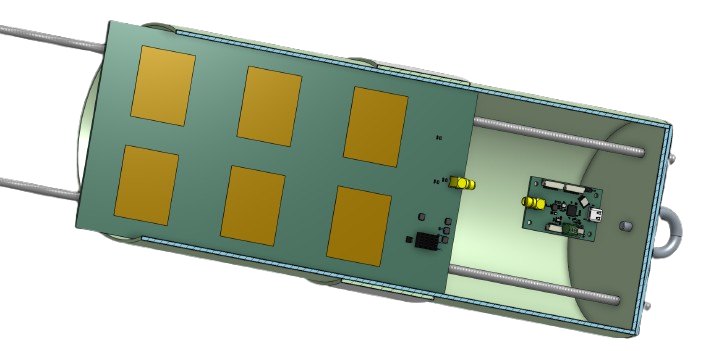
\includegraphics[width=.75\linewidth]{Documentation/ARES/Use_Cases/Pics/PHOBOS_Cad.png}
    \caption{\phobos{} System CAD model showing the antenna array board and central controlling board inside the ARES canister.}
    \label{fig:PHOBOS_CAD}
\end{figure}